\documentclass[handout]{beamer}  

%Smaller gap at between top and bottom of block when there are displayed equations
\addtobeamertemplate{block begin}{\setlength\abovedisplayskip{0pt}}
{\setlength{\belowdisplayskip}{0pt}}


\usepackage{setspace}
\linespread{1.3}
\usepackage{amssymb, amsmath, amsthm} 
\usepackage{rotating}
\usepackage{multirow}
\usepackage{graphicx}
\usepackage{synttree}
\usepackage{verbatim}
\usepackage{fancybox}
\usepackage{color}
\usepackage{tikz}
\usetikzlibrary{shapes,backgrounds}
\usepackage{hyperref}
\usetikzlibrary{trees}
\newcommand{\p}{\mathbb{P}}
\newcommand{\expect}{\mathbb{E}}


%\setbeamertemplate{blocks}[rounded][shadow=true] 
%gets rid of bottom navigation bars
\setbeamertemplate{footline}{
   \begin{beamercolorbox}[ht=4ex,leftskip=0.3cm,rightskip=0.3cm]{author in head/foot}
%    \usebeamercolor{UniBlue}
    \vspace{0.1cm}
    %\insertshorttitle \ - \insertdate 
    \hfill \insertframenumber / \inserttotalframenumber
   \end{beamercolorbox}
   \vspace*{0.1cm}
} 


%gets rid of navigation symbols
\setbeamertemplate{navigation symbols}{}


%Include or exclude the notes?
%\setbeameroption{show notes}
\setbeameroption{hide notes}


\title[Econ 103]{Economics 103 -- Statistics for Economists} 
\author[F. DiTraglia]{Francis J.\ DiTraglia}
\institute{University of Pennsylvania}
\date{Lecture 9}
\begin{document} 
%%%%%%%%%%%%%%%%%%%%%%%%%%%%%%%%%%%%%%%%

\begin{frame}[plain]
	\titlepage 
	

\end{frame} 
%%%%%%%%%%%%%%%%%%%%%%%%%%%%%%%%%%%%%%%%

\begin{frame}
\centering \Huge Discrete RVs -- Part II

\end{frame}


%%%%%%%%%%%%%%%%%%%%%%%%%%%%%%%%%%%%%%%%

\begin{frame}
\frametitle{Last Time}
\begin{block}{Random Variable (RV)}
$X\colon S \mapsto \mathbb{R}$
\end{block}
\begin{block}{Probability Mass Function (pmf)}
$p(x) = P(X = x)$
\end{block}
\begin{block}{Cumulative Distribution Function (CDF)}
$F(x_0) = P(X \leq x_0)$
\end{block}
\begin{block}{Expected Value (aka Expectation/Mean)}
$\mu = E[X] = \displaystyle\sum_{\mbox{all } x} x \cdot p(x)$
\end{block}
\end{frame}


%%%%%%%%%%%%%%%%%%%%%%%%%%%%%%%%%%%%%%%%

% \begin{frame}
% \frametitle{Last Time}

% \begin{block}{Expected Value (aka Expectation)}
% For a discrete RV, the the \alert{probability-weighted average} of all realizations	
% $$E[X] = \sum_{\mbox{all} \; x} x \cdot p(x)$$
% \end{block}	

% \begin{block}{Population Model}
% 	If the RV $X$ is a probability model for some population, we equate $E[X]$ with the population mean $\mu$.
% \end{block}
	
% \end{frame}
% %%%%%%%%%%%%%%%%%%%%%%%%%%%%%%%%%%%%%%%%
% \begin{frame}
% \frametitle{Last Time}

% \begin{block}{Expected Value of Bernoulli RV}
% 	$$X = \left\{ \begin{array}{l}  0, \mbox{Failure: } 1-p\\ 1, \mbox{Success: } p\end{array} \right.$$

% 	$$\sum_{\mbox{all} \; x} x \cdot p(x) = 0 \cdot (1-p) + 1 \cdot p = p$$
% \end{block}

% \end{frame}
%%%%%%%%%%%%%%%%%%%%%%%%%%%%%%%%%%%%%%%%
\begin{frame}
\frametitle{Today}
\begin{block}{More About Expected Value}
	\begin{itemize}
		\item Random Variables and Parameters
		\item Expectation of Functions
		\item Variance \& Standard Deviation
		\item Variance of Bernoulli RV
	\end{itemize}

\end{block}
\begin{block}{Binomial Random Variable}
\end{block}

\end{frame}
%%%%%%%%%%%%%%%%%%%%%%%%%%%%%%%%%%%%%%%%

\begin{frame}
\frametitle{Random Variables and Parameters}



\begin{block}{Notation: $X \sim$ Bernoulli$(p)$}
Means $X$ is a Bernoulli RV with $P(X = 1) = p$ and $P(X= 0) = 1-p$. The tilde is read ``distributes as.''

\end{block}


\begin{block}{Parameter}
Any constant that appears in the definition of a RV, here $p$. 
\end{block}


\begin{alertblock}{Important}
	Use RVs to model populations $\implies$ this definition of parameter corresponds to the one from earlier in the semester: a ``feature of the population (e.g.\ mean).''
\end{alertblock}


\end{frame}
%%%%%%%%%%%%%%%%%%%%%%%%%%%%%%%%%%%%%%%%

\begin{frame}
\frametitle{Constants Versus Random Variables}

 \alert{This is a crucial distinction that students sometimes miss:}
 \vspace{1em}
 

 		\begin{block}{Random Variables}
 			\begin{itemize}
 			\item Suppose $X$ is a RV -- the values it takes on are random
 			\item A function $g(X)$ of a RV is itself a RV as we'll learn today.
 			\end{itemize}
 		\end{block}
 
 		\begin{block}{Constants}
 			\begin{itemize}
 				\item $\mu = E[X]$ is a constant (you should convince yourself of this)
 				\item Realizations $x$ are constants. What is random is \emph{which} realization the RV takes on.
 				\item Parameters are constants (e.g.\ $p$ for Bernoulli RV)
 				\item Sample size $n$ is a constant
 			\end{itemize}
 		\end{block} 

\end{frame}
%%%%%%%%%%%%%%%%%%%%%%%%%%%%%%%%%%%%%%%%

\begin{frame}
\Huge \centering The St.\ Petersburg Game

\end{frame}
%%%%%%%%%%%%%%%%%%%%%%%%%%%%%%%%%%%%%%%%
\begin{frame}
\frametitle{How Much Would You Pay?\hfill 
\includegraphics[scale = 0.05]{./images/clicker}}
How much would you be willing to pay for the right to play the following game?

\vspace{1em}
\begin{quote}
Imagine a fair coin. The coin is tossed once. If it falls heads, you receive a prize of \$2 and the game stops. If not, it is tossed again. If it falls heads on the second toss, you get \$4 and the game stops. If not, it is tossed again. If it falls heads on the third toss, you get \$8 and the game stops, and so on. The game stops after the first head is thrown. If the first head is thrown on the $x^{th}$ toss, the prize is \$$2^x$
\end{quote}

\end{frame}
%%%%%%%%%%%%%%%%%%%%%%%%%%%%%%%%%%%%%%%%
\begin{frame}
\frametitle{$X =$ Trial Number of First Head}
\begin{table}
\begin{tabular}{c|c|c|c}
	$x$ & $2^x$ & $p(x)$& $2^x \cdot p(x)$\\
		\hline \uncover<2->{
	1&2&1/2&1\\
	2&4&1/4&1\\
	3&8&1/8&1\\}\uncover<3->{
	$\vdots$&$\vdots$&$\vdots$&$\vdots$\\
	n&$2^n$&$1/2^n$&1\\
	$\vdots$&$\vdots$&$\vdots$&$\vdots$}
\end{tabular}
\end{table}
$$E[Y] = \sum_{\mbox{all } x} 2^x\cdot p(x) = \uncover<4->{1 + 1 + 1 + \hdots}\uncover<5->{ = \infty}$$
\end{frame}
%%%%%%%%%%%%%%%%%%%%%%%%%%%%%%%%%%%%%%%%

\begin{frame}
\begin{center}
\Huge Functions of Random Variables are Themselves Random Variables
\end{center}

\end{frame}
%%%%%%%%%%%%%%%%%%%%%%%%%%%%%%%%%%%%%%%%

\begin{frame}
\frametitle{Example: Function of Bernoulli RV}
\fbox{Let $Y=e^X$ where $X \sim \mbox{Bernoulli}(p)$}
\vspace{2em}

\begin{block}{Support of $Y$} \pause
$\{e^0, e^1\} =\{1, e\}$
\end{block}

\begin{block}{Probability Mass Function for $Y$} \pause
	$$p_Y(y) = \left\{\begin{array}{ll}p& y =e\\ 1-p& y = 1\\ 0& \mbox{otherwise}\end{array}\right.$$
\end{block}

\end{frame}
%%%%%%%%%%%%%%%%%%%%%%%%%%%%%%%%%%%%%%%%
\begin{frame}
\frametitle{Expectation: Function of Bernoulli RV}
\fbox{Let $Y=e^X$ where $X \sim \mbox{Bernoulli}(p)$}
\vspace{2em}

\begin{block}{Probability Mass Function for $Y$} 
	$$p_Y(y) = \left\{\begin{array}{ll}p& y =e\\ 1-p& y = 1\\ 0& \mbox{otherwise}\end{array}\right.$$
\end{block}

\begin{block}{Expectation of $Y = e^X$}\pause
$$\sum_{y \in \{1, e\}} y \cdot p_Y(y) =\pause (1-p) \cdot 1 + p \cdot e = 1 + p(e - 1)$$
\end{block}




\end{frame}
%%%%%%%%%%%%%%%%%%%%%%%%%%%%%%%%%%%%%%%%
\begin{frame}
\frametitle{Expectation: Function of Bernoulli RV}
\fbox{Let $Y=e^X$ where $X \sim \mbox{Bernoulli}(p)$}
\vspace{2em}



\begin{block}{Expectation of the Function}
$$\sum_{y \in \{1, e\}} y \cdot p_Y(y) = (1-p) \cdot 1 + p \cdot e = 1 + p(e - 1)$$
\end{block}

\begin{block}{Function of the Expectation}
$$e^{E[X]} = e^p $$
\end{block}



\end{frame}
%%%%%%%%%%%%%%%%%%%%%%%%%%%%%%%%%%%%%%%%


\begin{frame}
\huge $$E[g(X)] \neq g(E[X])$$
\begin{center}
	\large (Expected value of Function $\neq$ Function of Expected Value)
\end{center}


\end{frame}
%%%%%%%%%%%%%%%%%%%%%%%%%%%%%%%%%%%%%%%%

\begin{frame}
\frametitle{Expectation of a Function of a Discrete RV}
Let $X$ be a random variable and $g$ be a function. Then:
$$\boxed{E[g(X)] = \sum_{\mbox{all } x} g(x) p(x)}$$


 \alert{This is how we proceeded in the St.\ Petersburg Game Example}
\end{frame}
%%%%%%%%%%%%%%%%%%%%%%%%%%%%%%%%%%%%%%%%
\begin{frame}
\frametitle{Your Turn: Calculate $E[X^2]$ \hfill 
\includegraphics[scale = 0.05]{./images/clicker}}
$X$ has support $\{-1, 0, 1\}$, $p(-1) = p(0) = p(1) = 1/3$.
\pause

\begin{eqnarray*}
 E[X^2] &=&  \sum_{\mbox{all } x} x^2 p(x) = \sum_{x \in \{-1, 0, 1\}} x^2 p(x) \\ \\ \pause
 	&=& (-1)^2 \cdot (1/3) + (0)^2 \cdot (1/3) + (1)^2 \cdot (1/3)\\ \pause
 	&=& 1/3 + 1/3\\ 
 	&=& 2/3 \approx 0.67
\end{eqnarray*}

\end{frame}
%%%%%%%%%%%%%%%%%%%%%%%%%%%%%%%%%%%%%%%%

\begin{frame}
\frametitle{Linearity of Expectation}
\framesubtitle{Holds for Continuous RVs as well, but proof is different.}
Let $X$ be a RV and $a,b$ be constants. Then:
	$$E[a + bX] = a + bE[X]$$
\vspace{2em}
\begin{alertblock}{This is one of the most important facts in the course: the special case in which $E[g(X)] = g(E[X])$ is $g = a+bX$.}
\end{alertblock}
\end{frame}
%%%%%%%%%%%%%%%%%%%%%%%%%%%%%%%%%%%%%%%%
\begin{frame}
\frametitle{Proof: Linearity of Expectation For Discrete RV}

\begin{eqnarray*}
	E[a + bX] &=& \pause \sum_{\mbox{all } x}  (a + bx) p(x)\\ \\
	 &=&\pause  \sum_{\mbox{all } x} p(x) \cdot a + \sum_{\mbox{all } x}p(x) \cdot bx\\ \\
	&=& \pause a\sum_{\mbox{all } x} p(x) + b\sum_{\mbox{all } x} x \cdot p(x) \\ \\
	&=& \pause a + b E[X]
\end{eqnarray*}


\end{frame}
%%%%%%%%%%%%%%%%%%%%%%%%%%%%%%%%%%%%%%%%

\begin{frame}
\frametitle{Variance and Standard Deviation of a RV}
\framesubtitle{The Defs are the same for continuous RVs, but the method of calculating will differ.}

\begin{block}{Variance (Var)}
	$$\sigma^2 = Var(X) = E\left[ (X - \mu)^2\right] = E\left[ (X - E[X])^2\right]$$
\end{block}
\pause

\begin{block}{Standard Deviation (SD)}
$$\sigma = \sqrt{\sigma^2} = SD(X)$$
\end{block}


\end{frame}
%%%%%%%%%%%%%%%%%%%%%%%%%%%%%%%%%%%%%%%%
\begin{frame}
\frametitle{Key Point}

\alert{Variance and std.\ dev.\ are \emph{expectations of functions of a RV}} 

\vspace{1em}

It follows that: 
\begin{enumerate}
\item Variance and SD are constants
\item To derive facts about them you can use the facts you know about expected value
\end{enumerate}
\end{frame}
%%%%%%%%%%%%%%%%%%%%%%%%%%%%%%%%%%%%%%%%
\begin{frame}
\frametitle{How To Calculate Variance for Discrete RV?}
\framesubtitle{Remember: it's just a function of $X$!}


Recall that	$\displaystyle \mu = E[X] = \sum_{\mbox{all } x} xp(x)$

\pause
\vspace{3em}

$$Var(X) = E\left[ (X - \mu)^2 \right] =\sum_{\mbox{all } x} (x - \mu)^2 p(x)$$


\end{frame}
%%%%%%%%%%%%%%%%%%%%%%%%%%%%%%%%%%%%%%%%
\begin{frame}
\frametitle{Shortcut Formula For Variance}

This is \emph{not} the definition, it's a shortcut for doing calculations:
\begin{eqnarray*}
	Var(X) = E\left[ (X - \mu)^2 \right] = E[X^2] - \left(E[X]\right)^2
\end{eqnarray*}

\alert{We'll prove this next week.}

\end{frame}

%%%%%%%%%%%%%%%%%%%%%%%%%%%%%%%%%%%%%%%%


\begin{frame}
\frametitle{Variance of Bernoulli RV -- via the Shortcut Formula}

\begin{block}{Step 1 -- $E[X]$} \pause
$\mu = E[X] = \displaystyle \sum_{x \in \{0,1\}} p(x) \cdot x = (1-p) \cdot 0 + p \cdot 1 = p$
\end{block}

\begin{block}{Step 2 -- $E[X^2]$} \pause
\begin{eqnarray*}
	E[X^2] = \sum_{x \in \{0,1\}} x^2 p(x) = 0^2 (1-p) + 1^2 p = p
\end{eqnarray*}
\end{block}

\begin{block}{Step 3 -- Combine with Shortcut Formula} \pause
\begin{eqnarray*}
	\sigma^2 = Var[X] = E[X^2] - \left(E[X]\right)^2 = \pause p - p^2 = \pause p(1-p)
\end{eqnarray*}
\end{block}


\end{frame}
%%%%%%%%%%%%%%%%%%%%%%%%%%%%%%%%%%%%%%%%



\begin{frame}
\frametitle{Variance of Bernoulli RV -- Without Shortcut}

\alert{You will fill in the missing on the problem set...}

\begin{eqnarray*}
	\sigma^2 &=& Var(X) = \sum_{x \in \{0,1\}} (x - \mu)^2 p(x)\\
	 &=& \sum_{x \in \{0,1\}} (x - p)^2 p(x)\\
	 &\vdots &\\ 
	 &=&p(1-p)
\end{eqnarray*}

%%%%%%%%%%%%%%%%%%%%%%%%%%%%%%%%%%%%%%%%


\end{frame}

\begin{frame}
\frametitle{Variance of a Linear Function  \hfill 
\includegraphics[scale = 0.05]{./images/clicker} }
Suppose $X$ is a random variable with $Var(X) = \sigma^2$ and $a,b$ are constants. What is $Var(a + bX)$? 
\begin{enumerate}[(a)]
	\item $\sigma^2$
	\item $a + \sigma^2$
	\item $b \sigma^2$
	\item $a + b \sigma^2$
	\item $b^2 \sigma^2$
\end{enumerate}

\end{frame}
%%%%%%%%%%%%%%%%%%%%%%%%%%%%%%%%%%%%%%%%
\begin{frame}
	\frametitle{Variance and SD are \emph{NOT} Linear}

\begin{eqnarray*}
Var(a + bX) &= &b^2 \sigma^2 \\\\
	SD(a + bX)&=& b \sigma
\end{eqnarray*}

\vspace{2em}
\begin{block}{These should look familiar from the related results for sample variance and std.\ dev. that you worked out on an earlier problem set.}

\end{block}

\end{frame}
%%%%%%%%%%%%%%%%%%%%%%%%%%%%%%%%%%%%%%%%
\begin{frame}
\frametitle{Variance of a Linear Transformation}

\begin{eqnarray*}
 Var(a + bX) &=& E\left[\left\{(a+bX) - E(a+bX)\right\}^2 \right] \\ \pause
 	&=& E\left[\left\{(a+bX) - (a+bE[X])\right\}^2 \right] \\ \pause
 	&=&E\left[\left(bX - bE[X]\right)^2 \right] \\ \pause
 	&=&E[b^2 (X - E[X])^2]\\ \pause
 	&=& b^2 E[(X-E[X])^2]\\ \pause
 	&=& b^2 Var(X) = b^2 \sigma^2
\end{eqnarray*}
\alert{The key point here is that variance is defined in terms of expectation and expectation is linear.}

\end{frame}
%%%%%%%%%%%%%%%%%%%%%%%%%%%%%%%%%%%%%%%%
\begin{frame}
	\begin{center}
		\Huge Binomial Random Variable	\\
		\large What we get if we sum a bunch of indep.\ Bernoulli RVs
	\end{center}
\end{frame}

%%%%%%%%%%%%%%%%%%%%%%%%%%%%%%%%%%%%%%%%

\begin{frame}
\frametitle{
\includegraphics[scale = 0.05]{./images/clicker} }
\begin{block}{Question}
Suppose we flip a fair coin 3 times. What is the probability that we get exactly 2 heads?
\end{block}

\pause

\begin{block}{Answer}
Three basic outcomes make up this event: $\{HHT, HTH, THH\}$. \pause Each of these has probability $1/8 = 1/2 \times 1/2 \times 1/2$ so, since basic outcomes are mutually exclusive we sum to get \pause \alert{$3/8 = 0.375$}
\end{block}

\end{frame}
%%%%%%%%%%%%%%%%%%%%%%%%%%%%%%%%%%%%%%%%
\begin{frame}
\frametitle{A More Complicated Example}
\begin{block}{Question}
Suppose we flip an \emph{unfair} coin 3 times, where the probability of heads is 1/3. What is the probability that we get exactly 2 heads?
\end{block}

\pause

\begin{block}{Answer}
The basic outcomes of the experiment are no longer equally likely, but those with exactly two heads \emph{\alert{remain so}} \pause
	\begin{eqnarray*}
	 P(HHT) &=&  (1/3)^2 (1 - 1/3) =  2/27\\ \pause
	 P(THH) &=&2/27\\ \pause
	 P(HTH) &=&2/27 \pause
	\end{eqnarray*}
	Summing gives \alert{$2/9 \approx 0.22$}
\end{block}
\end{frame}
%%%%%%%%%%%%%%%%%%%%%%%%%%%%%%%%%%%%%%%%
\begin{frame}
\frametitle{Starting to see a pattern?}

Suppose we flip an unfair coin \emph{4} times, where the probability of heads is 1/3. What is the probability that we get exactly 2 heads?

\vspace{2em}

\pause

\begin{columns}
\column{0.35\textwidth}
\begin{tabular}{cc}
HHTT&TTHH\\
HTHT&THTH\\
HTTH&THHT
\end{tabular}

\column{0.55\textwidth}
\alert{Six equally likely, mutually exclusive basic outcomes make up this event:}
$${4\choose 2}(1/3)^2(2/3)^2$$
\end{columns}

\end{frame}

%%%%%%%%%%%%%%%%%%%%%%%%%%%%%%%%%%%%%%%%

\begin{frame}
\frametitle{Binomial Random Variable}
Let $X = $ the sum of $n$ independent Bernoulli trials, each with probability of success $p$. \pause \alert{Then we say that:
		$X \sim \mbox{Binomial}(n,p)$} \pause

\vspace{2em}
\begin{block}{Parameters}\pause
$p =$ probability of ``success,'' $n=$ \# of trials
\end{block}\pause
\begin{block}{Support} \pause
$\{0, 1, 2, \hdots, n\}$ \pause
\end{block}
\begin{block}{Probability Mass Function (pmf)} \pause
$$p(x) = {n \choose x} p^x (1-p)^{n-x}$$ 
\end{block}
\end{frame}
%%%%%%%%%%%%%%%%%%%%%%%%%%%%%%%%%%%%%%%%

\begin{frame}
	\frametitle{\href{http://glimmer.rstudio.com/fditraglia/binom_cdf/}{http://glimmer.rstudio.com/fditraglia/binom\_cdf/}}
\framesubtitle{Try playing around with all three sliders. If you set the second to 1 you get a Bernoulli.}

\begin{figure}
	\fbox{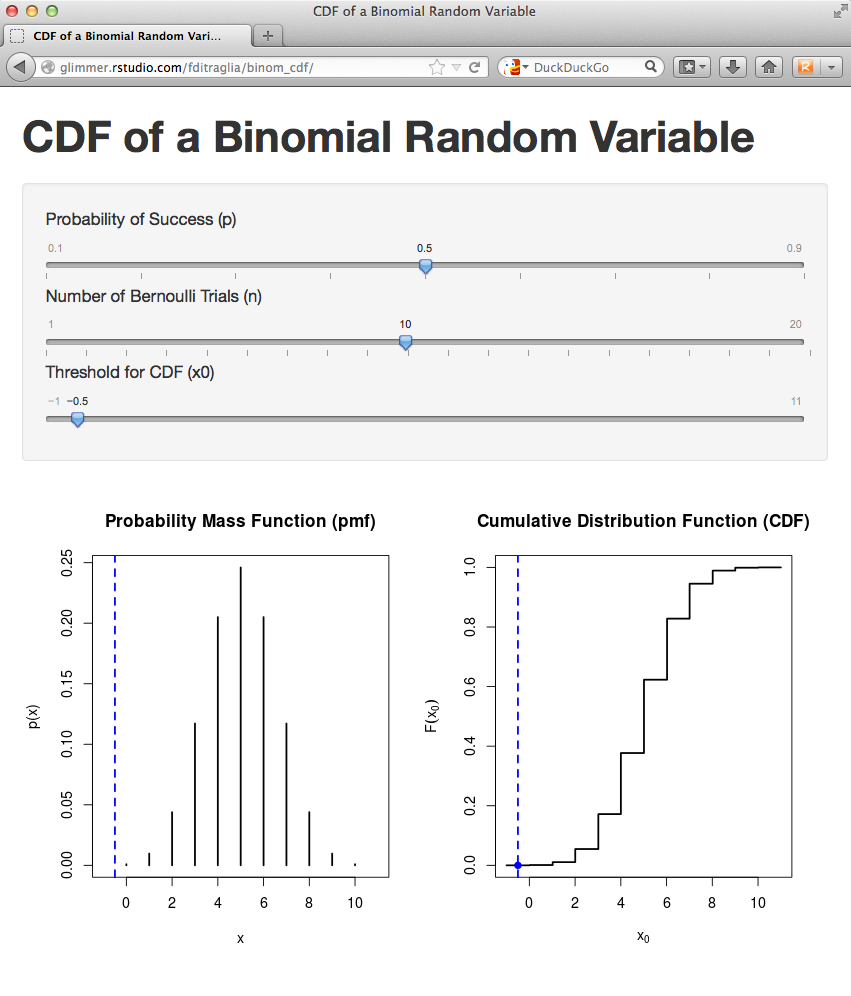
\includegraphics[scale = 0.2]{./images/binom_cdf_screenshot2}}
\end{figure}

\end{frame}

%%%%%%%%%%%%%%%%%%%%%%%%%%%%%%%%%%%%%%%%



\begin{frame}
\frametitle{Don't forget this!}
 \large A Binomial Random Variable counts up the \emph{total} number of successes (ones) in $n$ independent Bernoulli trials, each with probability of success $p$.


\vspace{5em}
\alert{We'll learn more about the Binomial RV in the coming lectures...}
\end{frame}
%%%%%%%%%%%%%%%%%%%%%%%%%%%%%%%%%%%%%%%%

\begin{frame}
	\frametitle{\href{http://ditraglia.com/econ103/Bernoulli_Binomial.html}{http://ditraglia.com/econ103/Bernoulli\_Binomial.html}}
\framesubtitle{Source Code on my \href{https://gist.github.com/fditraglia/7011503}{\fbox{Github Page}}}



\begin{figure}
	\fbox{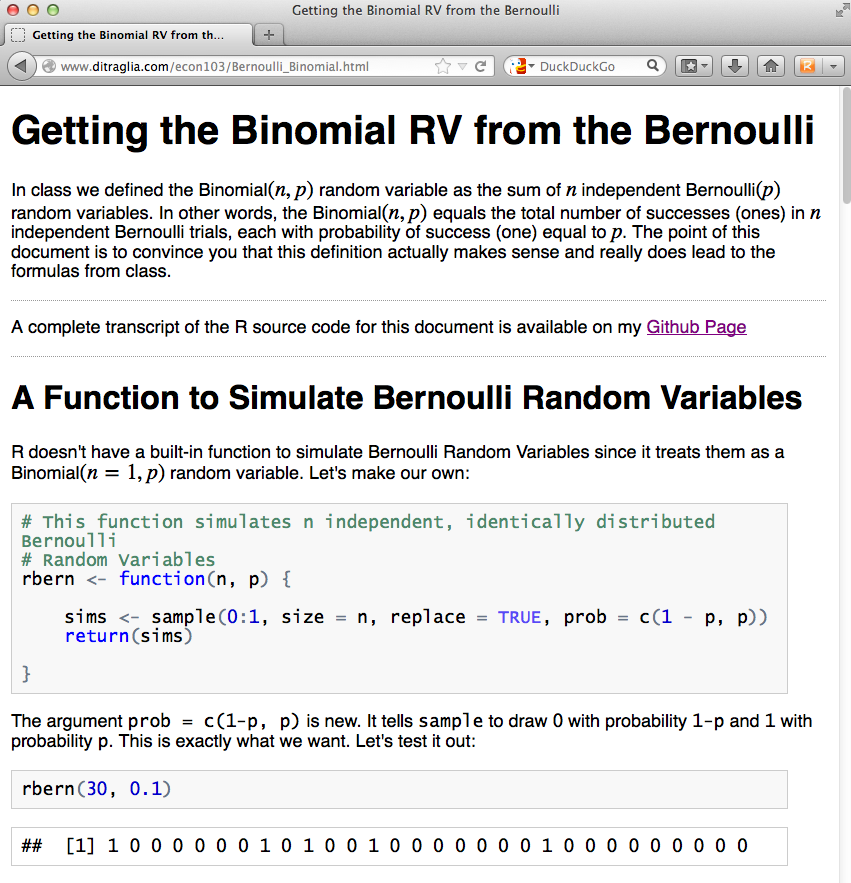
\includegraphics[scale = 0.2]{./images/binom_bernoulli_sim_screenshot}}
\end{figure}

\end{frame}

%%%%%%%%%%%%%%%%%%%%%%%%%%%%%%%%%%%%%%%%

% \begin{frame}
% \frametitle{Binomial pmfs for Assorted Parameter Values}
% \begin{figure}
% \centering
% 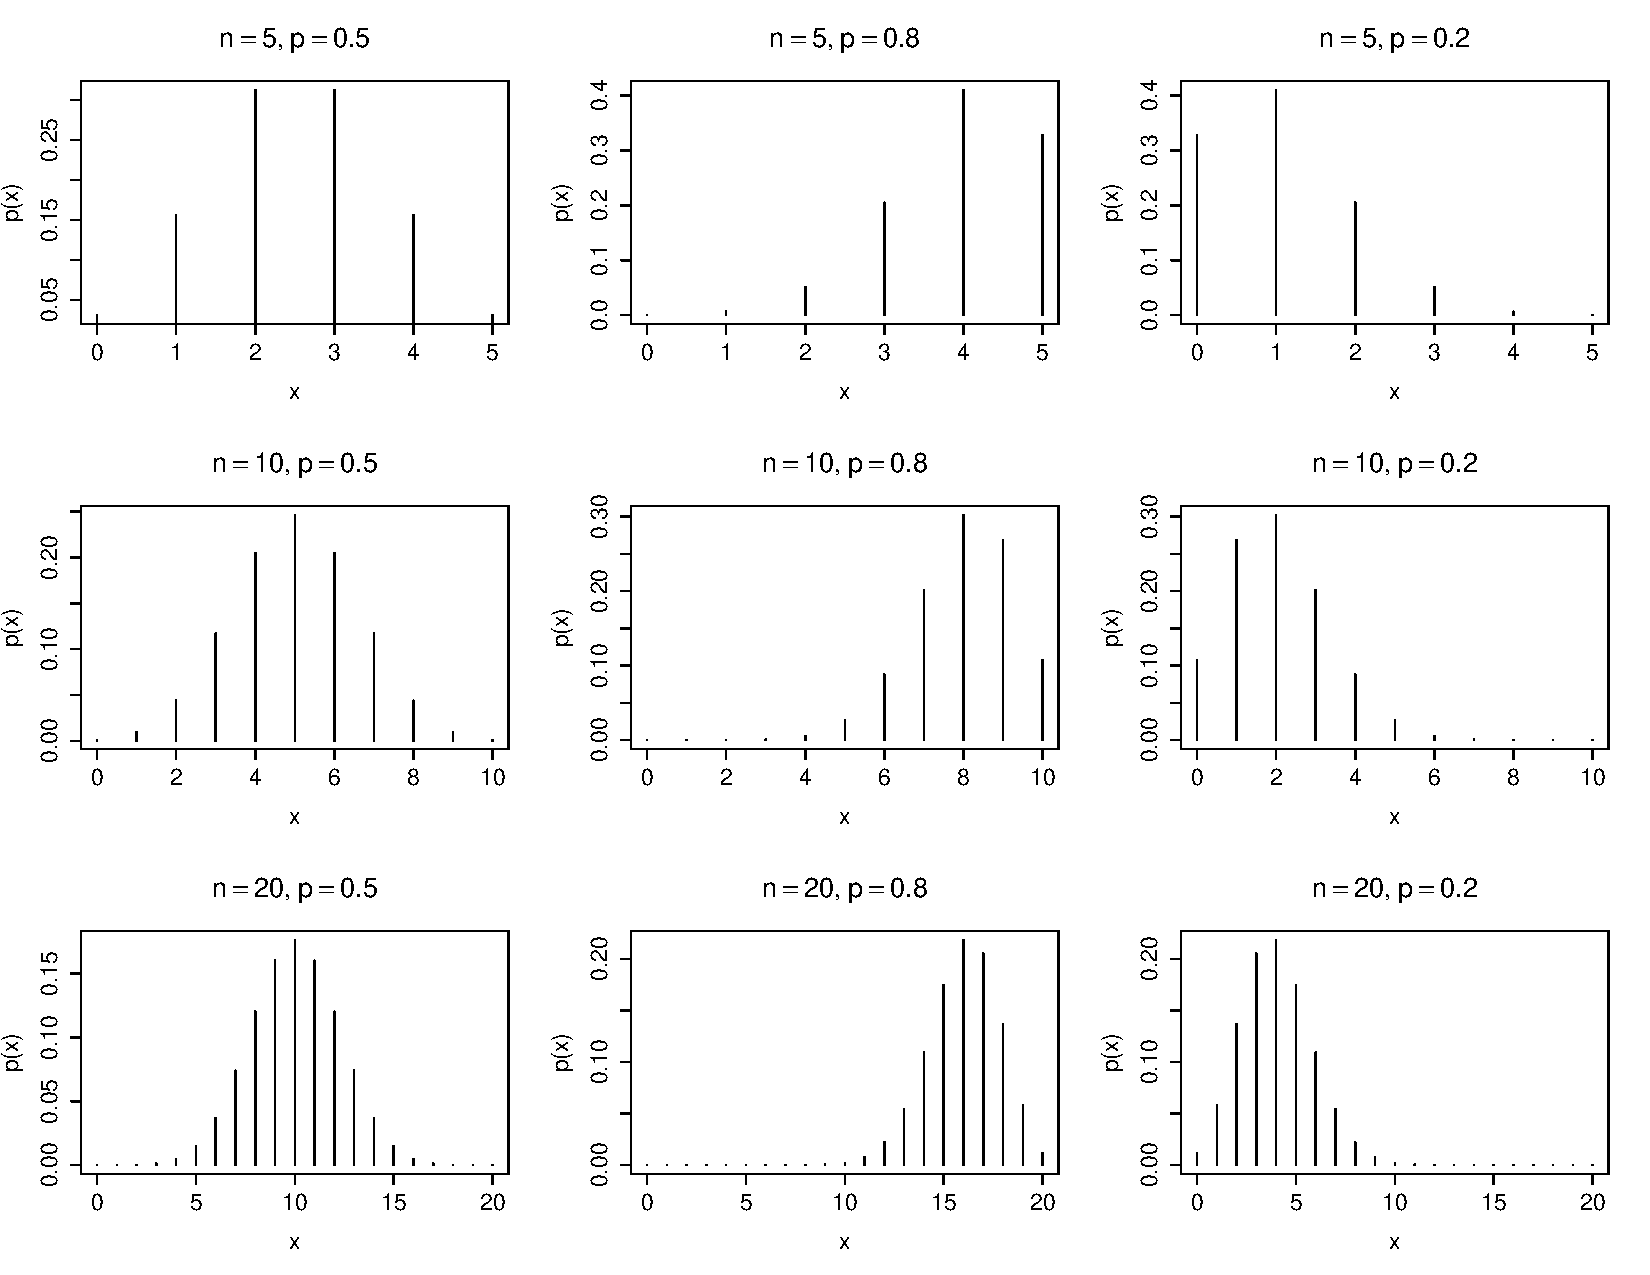
\includegraphics[scale=0.35]{./images/binom_pmfs}
% \end{figure}
% \end{frame}
% %%%%%%%%%%%%%%%%%%%%%%%%%%%%%%%%%%%%%%%%
% \begin{frame}
% \frametitle{Corresponding Binomial CDFs}
% \begin{figure}
% \centering
% 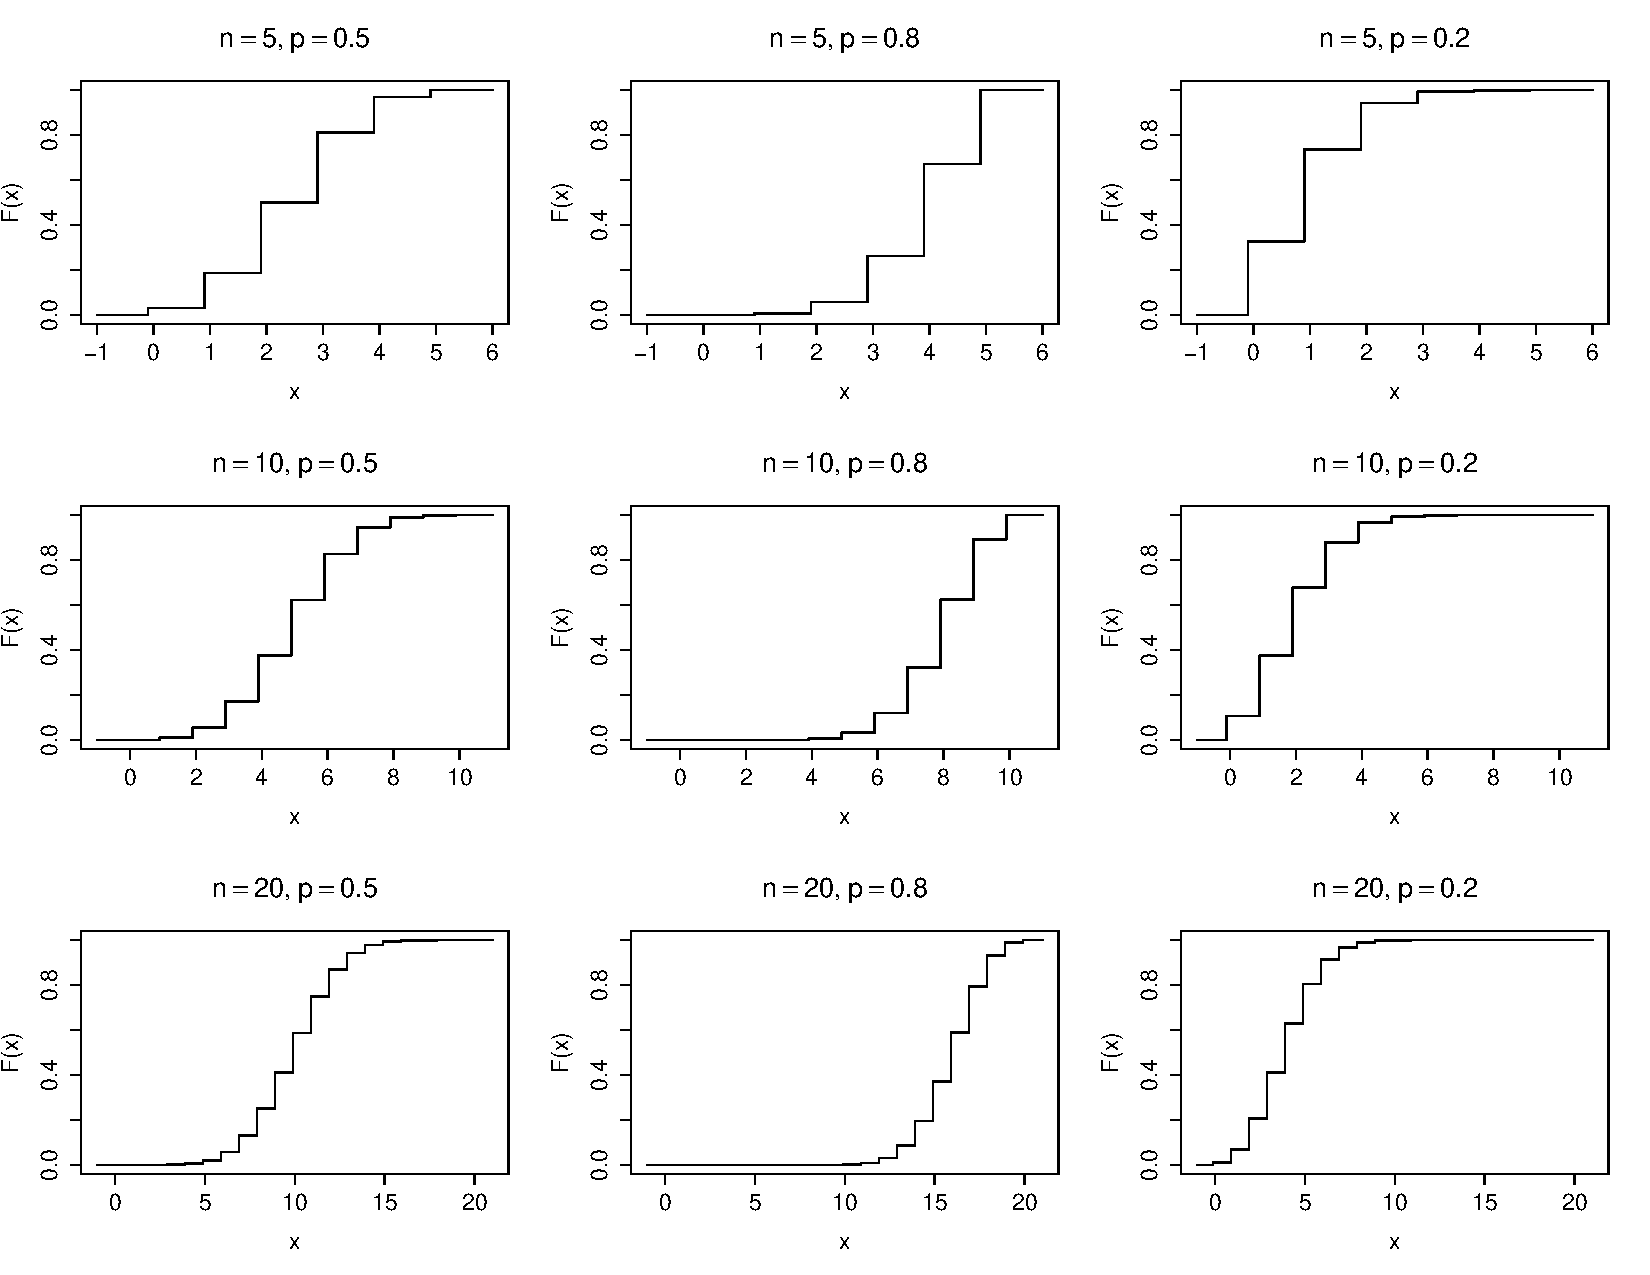
\includegraphics[scale=0.35]{./images/binom_cdfs}
% \end{figure}
% \end{frame}
% %%%%%%%%%%%%%%%%%%%%%%%%%%%%%%%%%%%%%%%%
%\begin{frame}
%\frametitle{Binomial Gives a Model for Polling a Random Sample}
%
%\begin{itemize}
%	\item Suppose a fraction $p$ of the US population supports gay marriage and you poll a random sample of size $n$. \pause
%	\item Binomial pmf lets you work out the probability of any outcome of your poll in terms of $n$ and $p$. \pause
%	\item If $n$ is large, the proportion who support gay marriage in your \alert{\alert{sample}} is very unlikely to be far from $p$, the true \alert{population} proportion.
%\end{itemize}
% 
% \pause
%\hfill\alert{We'll learn more about the Binomial RV next week...}
%\end{frame}
%%%%%%%%%%%%%%%%%%%%%%%%%%%%%%%%%%%%%%%%




\end{document}
